\documentclass[10pt, twoside]{article}
\usepackage[utf8]{inputenc}
\usepackage{graphicx} % Required for inserting images
\usepackage{amsmath}
\usepackage{amssymb}
\usepackage[a4paper,left=2.1cm, right=2.1cm, top=2cm, bottom=2cm]{geometry}
\usepackage{verbatim}
\usepackage[english]{babel}
\usepackage{hyperref}
\usepackage{listings}
\usepackage{float}
\usepackage{xcolor}
\definecolor{boxgray}{RGB}{230,230,230}
\renewcommand{\arraystretch}{1.5}
\setlength{\tabcolsep}{0.24cm}

\usepackage{comment}
\renewcommand{\rmdefault}{cmss}
\newcommand{\ttt}[1]{\colorbox{boxgray}{\texttt{#1}}}
\lstdefinestyle{mystyle}{	basicstyle=\ttfamily\footnotesize
}

\lstset{style=mystyle}

\title{ROOT}
\author{Pocket reference for 1st and 2nd year courses - BSc Physics, Unibo}
\date{2023-2024}

\begin{document}
\maketitle
{\small\tableofcontents}
\hfill
\begin{center}
\textbf{A general note:} strings between \ttt{<} ... \ttt{>} are meant to be replaced by suitable ones (without the two kets)
\end{center}
\hfill

\section{General structure}

ROOT contains \textbf{interpreter} : \textit{Just-In-Time} compilation $\rightarrow$ prompt : special commands (not standard C++ syntax) with \boxed{\texttt{.}}.

Base class \ttt{TObject} $\rightarrow$ \ttt{TNamed} $\rightarrow$ \ttt{TH1} (histograms) $\rightarrow$ \ttt{TH1F, TH1D, THIC, TH1S} according to \textbf{type representing entries} (not the type of data!!)

\section{Basic shell \& prompt commands}
! Possible to use \boxed{Tab}
\begin{itemize}
\item \boxed{\texttt{root}} launch ROOT
\item \boxed{\texttt{.q}} quit
\item \boxed{\texttt{.L <file.C>}} load file (symbols defined in a macro)
\item \boxed{\texttt{.help}} \boxed{\texttt{.?}} full help list
\item \boxed{\texttt{.! <cmd>}} call any shell command $<$cmd$>$ without leaving ROOT
\item \boxed{\texttt{.files}} shows loaded libraries / sources
\item \boxed{\texttt{.x <macro>}} loads \& runs a macro
\item \boxed{\texttt{.U <file.C>}} unload
\item \boxed{\texttt{.! wslview <image-file>}} (for WSL users) open image with default photo viewer from inside ROOT
\end{itemize}
Run a macro:
\begin{verbatim}
$ [0] .L <name>.C
$ [1] <name>()
\end{verbatim}
Load a library (class def) - only with \textbf{implementation file}:
\begin{verbatim}
$ [0] gROOT->LoadMacro(“MyClass.cxx+”)
\end{verbatim}
or
\begin{verbatim}
$ [0] .L MyClass.cxx+
\end{verbatim}
Produces a \textbf{dynamic library} file (\texttt{.so}). \\To automatically reload when running main macro put at beginning of latter:
\ttt{R\_\_LOAD\_LIBRARY( MyClass.so )}
\\~\\Possible to type C++ commands directly in shell: \textbf{';' are unnecessary, object type can be omitted in declarations, possible to access members with obj name instead than pointer}:
\begin{verbatim}
$ [0] TH1F *histo=new TH1F(“histname”,” Titolo”, 100, 0, 10)
$ [1] histname->Draw() // identical to histo->Draw()
\end{verbatim}
\textbf{Note:} \ttt{\#include <iostream>} and \ttt{namespace std;} are implicit!
\paragraph{Use prompt as calculator}
Ordinary operations + embedded library \ttt{TMath}:
\\\ttt{TMath::Abs(...), TMath::Exp(...), TMath::Gaus(...), TMath::Pi(), ...}
\subsection{Recover session history}
Saved in \ttt{\$/home/.root\_hist}

\subsection{Check versions}
\begin{description}
\item[\boxed{\texttt{gcc -v}}] gcc version
\item[\boxed{\texttt{lsb\_release -a}}] linux OS
\end{description}


\subsection{\LaTeX{}}
Can be used for labels etc. Same syntax as normal \LaTeX{}
\begin{itemize}
\item \verb^x_{1}^ = $x_1$
\item \verb_x^{1}_ = $x^1$
\end{itemize}
but commands are called with '\ttt{\#}' instead of '\ttt{\textbackslash}'

\section{Macros}
Two types of script
\paragraph{Unnamed script} all code between \{\} + no declaration of classes, functions + no parameters (ok loops)
\paragraph{Named script} like any C++ function + possible to define other functions, classes, use parameters
\\The executed function has the same name of the file (see Basics)

\section{GUI}
\boxed{\texttt{TBrowser b}} opens root files browser. 
\\Double click on an object (e.g. histo) $\rightarrow$ opens new \textbf{TCanvas} and draws it
\subsection*{Handling TCanvas}
if some of the followings not visible, click \textbf{View} and check out
\begin{description}
\item[Editor] single left click on an object in graph $\rightarrow$ edit display parameters (color etc.)
\item[Toolbar] tools to insert text, symbols, etc.
\item[Status bar] shows object pointed by mouse \& mouse position
\item Right click on object $\rightarrow$ contextual menu
\end{description}
\subsubsection*{Contextual menu}
\begin{description}
\item[Rebin] redefine binning
\item[Fit (of FitPanel)] fit a function on data (gaussian, exponential, polynomial etc.) $\rightarrow$ button \ttt{Set Parameters} for chosen distribution
\end{description}
To visualize fit on graph: right click on graph $\rightarrow$ open \ttt{TPaveStats::stats} $\rightarrow$ \ttt{SetOptFit} $\rightarrow$ se to \ttt{111}
\\\ttt{SetOptStat} allows do define other options
\paragraph{Canvas options} Right click on canvas $\rightarrow$ \ttt{SetLogx}, \ttt{SetLogy} for logarithmic scale; \ttt{SetGridx}, \ttt{SetGridy} for grid
\paragraph{Saving file} \ttt{File} $\blacktriangleright$ \ttt{Save} (\ttt{Save As})
\\Saving as \ttt{.C} file (containing the graph as C++ commands) enables to reproduce graph executing macro
\\Saving as \ttt{.root} file $\rightarrow$ saves canvas and all objects, double click on canvas inside .root (opened through TBrowser) to open and manipulate graph

\section{Global variables}
List of useful global pointers.
\begin{description}
\item[\ttt{gROOT}] global info on current session: access to \textbf{every object created during session}
\item[\ttt{gFile}] current root file
\item[\ttt{gStyle}] access functionalities to manage graphic style
\item[\ttt{gRandom}] access random number generator (see PRNG)
\item[\ttt{gPad}] current pad (see Canvas)
\end{description}
\paragraph{Suggestion} at the beginning of a macro, to eliminate copy created by multiple executions of code in a session: \ttt{delete gROOT->FindObject("<name>");}\\
\ttt{gROOT->FindObject("<name>")} used to retrieve every object from gROOT
\subsection*{General styling}
\ttt{gROOT->SetStyle("<style>");} set window style. Can be custom one or chosen between default ones:\\
\ttt{Classic, Plain, Modern, Bold, Video, Pub}

\section{Managing .root files}
\begin{description}
\item[\ttt{TFile *file = new TFile("<name>.root", "RECREATE");}] open file. Options:
\begin{description}
\item[\ttt{RECREATE}] creates new file if name not found, otherwise overwrites existing one
\item[\ttt{NEW}] or \ttt{CREATE} (error if already existing, returns empty ptr!) \item[\ttt{UPDATE}]
\item[\ttt{READ}] (default)
\end{description}
\item[\ttt{h->Write();}] write object (pointed by \ttt{h}) on file
\item[\ttt{file->Write();}] write all histos in memory in current session
\item[\ttt{file-ls();}] list content, with indentation for file tree
\item[\ttt{TH1F* hs = (TH1F*)file->Get("<name>");}] retrieve object from name
\\Explicit cast suggested
\item[\ttt{file->Close();}] close
\end{description}

\subsection{Decoupling from file}
To avoid disappearence of histos from canvas after closing read file(s):
\\\ttt{TH1::AddDirectory(kFALSE);} static! (default value is \texttt{kTrue})
\\\ttt{h->SetDirectory(0);} \ttt{h->DrawCopy();} non static

\subsection{Make user defined types writeable}
In header:
\begin{verbatim}
#ifndef MYCLASS_H 
#define MYCLASS_H
...
class MyClass: public TObject{
  public:
    ...
  private:
    ...
  ClassDef(MyClass,1)
};
#endif
\end{verbatim}
In implementation:
\begin{verbatim}
#include "MyClass.h"
...
ClassImp(MyClass)
\end{verbatim}

\section{TList}
A container class to store objects of every type inheriting from \texttt{TObject}

\begin{description}
\item[\ttt{TList * list= new TList();}]

\item[\ttt{list->Add(<ptr>);}] with pointer!

\item[\ttt{list->At(<idx>)}] indexing starts from 0, returns empty pointer if out of range

\item[\ttt{list->At(<idx>)->InheritsFrom("TGraph")}] check inheritance (boolean)
\end{description}

\section{Histograms}
\begin{description}
\item[1D]

\item[\ttt{TH1F* <pt-name> = new TH1F( "<name>", "<title>", <NxBins>, <xmin>, <xmax>);}] \,
\\declare new histogram
\\range [\ttt{xmin}, \ttt{xmax}] is equally subdivided in \ttt{N} bins

\item[\ttt{<pt-name>->Fill(<x>);}] fill histo with variable $<$x$>$ (e.g. from MC generation or read file, data)

\item[\ttt{<pt-name>->Fill(<x>, <n>);}] fill histo with n identical occurrences of x

\item[\ttt{<pt-name>->FillRandom("<funcname>",<Ntimes>,TRandom* rng = nullptr)}] fill \texttt{N} times generating according to auto normalized function (using \texttt{rng})

\item[\ttt{<pt-name>->Draw();}] draw histogram

\item[2D]

\item[\ttt{TH2F* <pt-name> = new TH2F( "<name>","<title>",<NxB>,<xmin>,<xmax>,<NyB>,<ymin>,<ymax>);}]

\item[\ttt{<pt-name>->Fill(x,y);}]
\item[\ttt{<pt-name>->Draw();}]

\item[\ttt{<pt-name>->ProjectionX()}] returns \texttt{TH1F} of projection w.r.t. x
\item[\ttt{<pt-name>->ProjectionY()}]
\item[\ttt{<pt-name>->GetNbinsX()}]
\item[\ttt{<pt-name>->GetNbinsY()}]

\item[3D]

\item[\ttt{TH3F* <pt-name> =}] \, \\
\ttt{new TH3F("<name>","<title>",<Nx>,<xmn>,<xmx>,<Ny>,<ymn>,<ymx>,<Nz>,<zmn>,<zmx>);}

\item[ND]

\item[\ttt{THnSparse* pt = new THSparse( "<name>", "<title>", <Ndims>, <xmin>, <xmax>, <chuncksize>);}] \,
\\min and max same for all dimensions
\end{description}

\subsection{Overlap histos}
\begin{verbatim}
// declare and initialize two histos, with pointers h1, h2
h1->Draw();
h2->Draw("same"); // or h2->Draw("SameHist");
\end{verbatim}

\subsection{Histo Draw options}
\begin{description}
\item[\ttt{"E"}] show error bars
\item[\ttt{"hist"}] show only histogram
\item[\ttt{"lego"}] lego plot
\item[\ttt{"cont"}] contour lines (linee di livello)
\item[\ttt{"Surf"}] surface
\item[\ttt{"P"}] draw marker (except empty bins)
\item[\ttt{"AXIS"}] draw only axis
\item[\ttt{"AXIG"}] draw only grid (if requested)
\item[\ttt{"FUNC"}]	When histo has fitted function, draw the fit result only.
\item[\ttt{"TEXT"}]	Draw bin contents as text (format set via 
\ttt{gStyle->SetPaintTextFormat}).
\item[\ttt{"X+"}]	The X-axis is drawn on the top side of the plot.
\item[\ttt{"Y+"}]	The Y-axis is drawn on the right side of the plot.
\item[\ttt{"MIN0"}] Set minimum value for the Y axis to $0$, equivalent to \ttt{gStyle->SetHistMinimumZero()}.
\end{description}
\boxed{\textbf{OPTIONS ARE NOT CASE SENSITIVE}}
\\~\\They can also be concatenated without spaces \& commas: \ttt{"opt1 opt2"}

\subsection{Cosmetics for histos}
\begin{description}
\item[\ttt{h1->SetMarkerStyle(<code>);}] set style, see $\downarrow$ for codes:
\begin{figure}[h!]
\centering
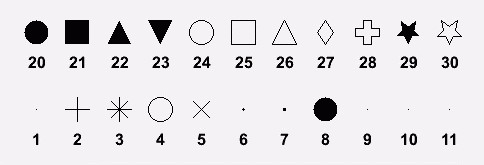
\includegraphics[scale=0.6]{imgs_root/shape.jpg}
\end{figure}
\item[\ttt{h1->SetMarkerSize(<rel\_sz>);}]
\item[\ttt{h1->GetXaxis()->SetTitle("<title>");}] change axis title, same for y with \ttt{GetYaxis()}
\item[\ttt{h1->GetXaxis()->SetTitleSize(<sz>);}] expressed as percent of pad size
\\\textbf{unless if precision = 3, when it's in pixels}
\item[\ttt{h1->GetXaxis()->SetTitleOffset(<ofs>);}] 0 is default, 1 is standard offset, 1.x adds 10*x\% 
\item[\ttt{SetFillColor(<color>);}] see after for codes
\item[\ttt{SetFillColorAlpha(<color>, <transparency ratio>);}] allows to manipulate opacity, \\e.g. \ttt{(kBlue, 0.35)}
\item[\ttt{SetLineColor(<color>);} or  \ttt{SetLineColorAlpha(<color>, <transp>);}]
\item[\ttt{SetLineStyle(<code>);}] see below
\item[\ttt{SetLineWidth(<width>);}] see below
\begin{figure}[H]
\centering
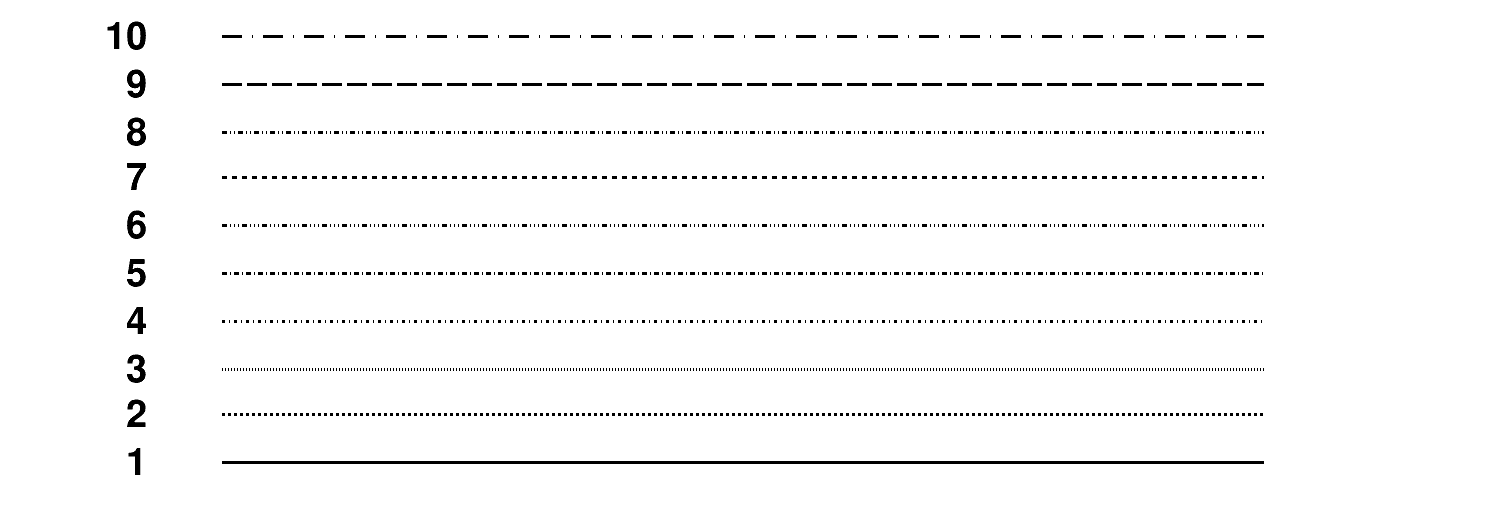
\includegraphics[scale=0.22]{imgs_root/linestyle.png}
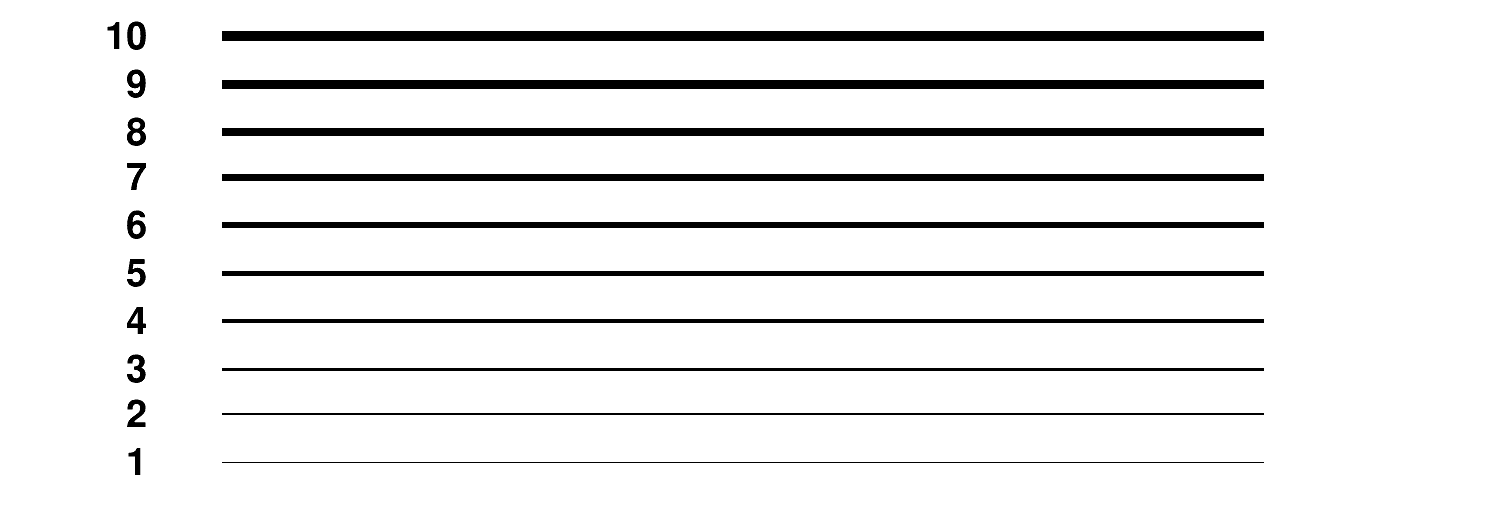
\includegraphics[scale=0.2]{imgs_root/linewidth.png}
\end{figure}
\item[\ttt{SetFillStyle(<code>);}] \textbf{0} for hollow, \textbf{1001} for solid, \textbf{3000 + pattern number} see below
\begin{figure}[h!]
\centering
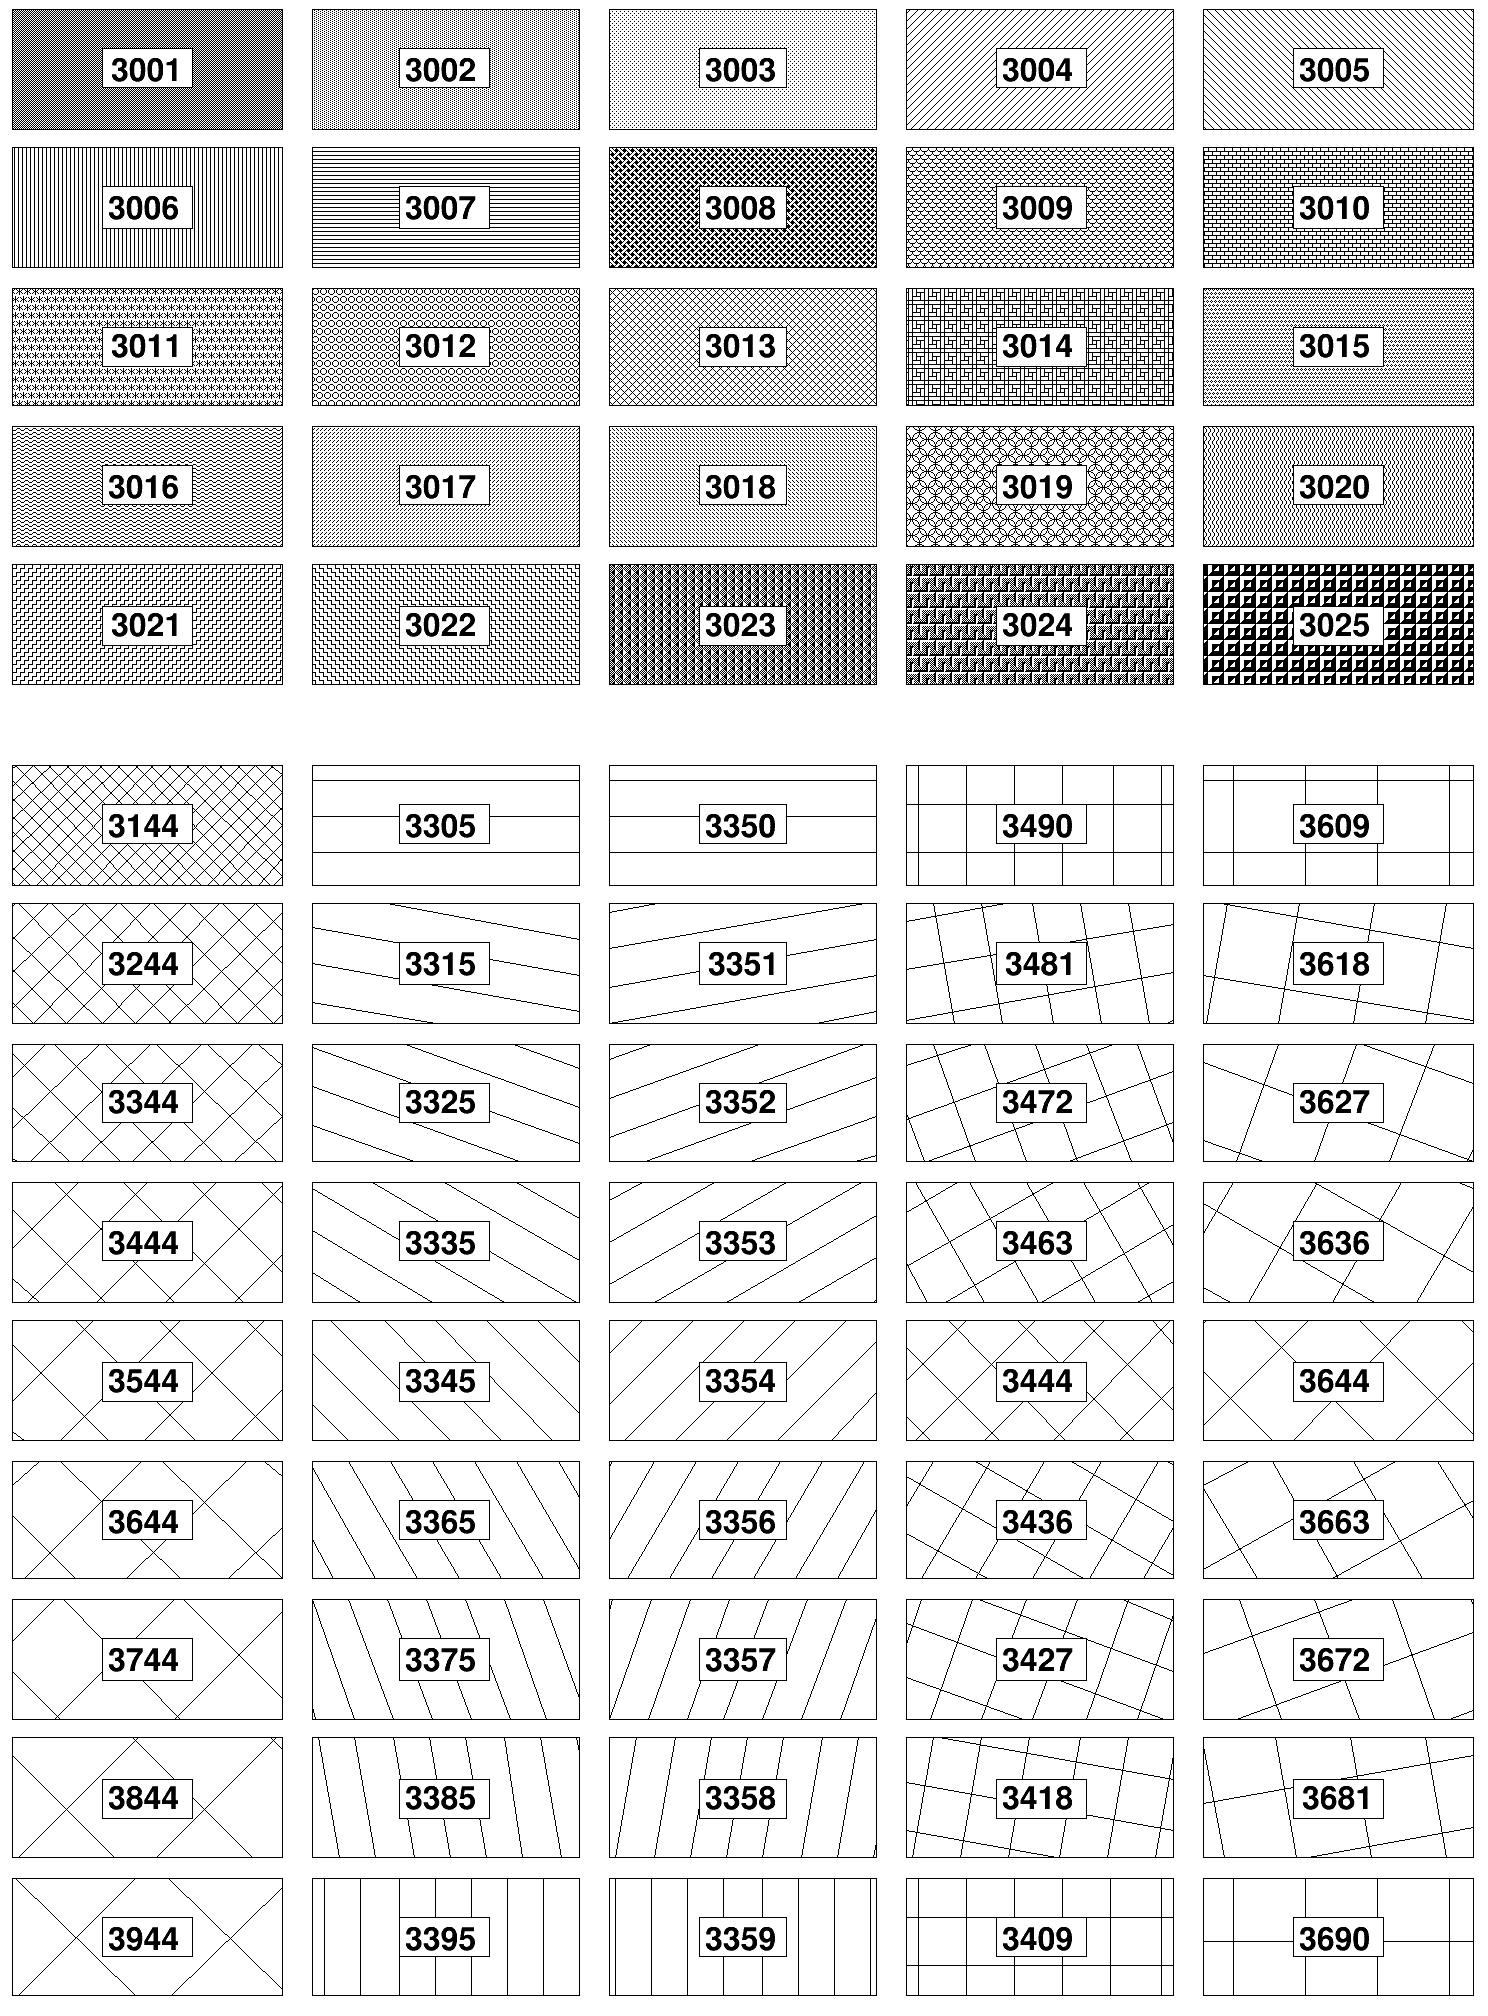
\includegraphics[scale=0.18]{imgs_root/fillstyles.png}
\end{figure}
\end{description}

\subsection{Other member functions for histos}
\begin{description}
\item[\ttt{GetMean()}] mean
\item[\ttt{GerRMS()} \ttt{GetStdDev()}] root of variance / SD
\item[\ttt{GetMaximum()}] maximum bin content
\item[\ttt{GetMaximumBin()}] location of maximum ($\neq$ former)
\item[\ttt{GetBinCenter( <bin\_number> )}] center of bin
\item[\ttt{GetBinContent( <bin\_number> )}] content of bin
\item[\ttt{GetBinError( <bin\_number> )}]
\item[\ttt{SetBinContent( <bin\_number>, <value> )}]
\item[\ttt{SetBinError( <bin\_number>, <value> )}]
\item[\ttt{GetNbinsX()}] number of bins
\end{description}
\textbf{Note:} for out-of-range entries:
\\\ttt{h->GetBinContent(0)} returns number of \textbf{underflow}
\\\ttt{h->GetBinContent(h->GetNbinsX()+ 1)} return number of \textbf{overflow}
\begin{description}
\item[\ttt{GetEntries()}] total entries (includes under/overflows)
\item[\ttt{Integral( <bin\_index1>, <bin\_index2> )}] integral on specified range
\item[\ttt{Integral()}] total integral
\item[\ttt{GetIntegral()}] array of cumulative entries
\item[\ttt{GetMeanError()}] error on mean estimate
\item[\ttt{GetRMSError()} \ttt{GetStdDevError()}] error on RMS estimate
\item[\ttt{Sumw2()}] create structure to store sum of square of weights. \textbf{Strongly suggested} before performing operations on histos
\end{description}

\subsection{Operations on histos}
Form homologue histograms (\textbf{same range and number of bins}): overloads for \textbf{istances}, \textbf{NOT POINTERS}:
\begin{verbatim}
TH1F h1;
TH1F h2 = 3*h1;
TH1F h3 = h1+h2;
\end{verbatim}
Otherwise through methods:

\begin{description}

\item[\ttt{h->Add(<pt1>, <pt2>, <n1>, <n2>);}] sum stored in *h, *h = n1*h1+n2*h2

\item[\ttt{h->Multiply(<int>);}]

\item[\ttt{h->Divide(<pt1>, <pt2>, <n1>, <n2>);}] analogous to sum

\end{description}

\subsection{Filling a histo from ascii file}
\begin{verbatim}
TH1F *h1 = new TH1F("h1","Tempi di Caduta",8,-0.5,15.5); 

ifstream in;
in.open("maxwell.dat");
Float_t x,y;
while (1) { // always true condition: iterates until break called
   in >> x >> y;
   if(!in.good()) break;
   h1->Fill(y);
}
in.close();
\end{verbatim}

\section{Graphs}
Two classes: \textbf{\ttt{TGraph}} (series of N X-Y couples), \textbf{\ttt{TGraphErrors}} (derived from former, includes also errors on both X and Y)

\paragraph{TGraph Constructors} Derived class!
\begin{description}
\item[\ttt{TGraph (<int\_N>, <db*\_x>, <db*\_y>)}] \texttt{N} couples, \ttt{x} and \ttt{y} are \textbf{arrays} of size \texttt{N}
\item[\ttt{TGraph (const char *filename, const char *format="\%lg \%lg", 
Option\_t *option="")}] input file \textbf{must contain 2 separate columns of values} (divided by blank delimiter) 
\\Default format: \ttt{"\%lg \%lg"} (2 double)\\
To skip columns: \ttt{\%lg \%*lg \%lg"}
\\Additional options to interpret different delimiters: explicitly specified in option argument ( \ttt{option = "<symbol>"} )
\end{description}
\paragraph{TGraphErrors Constructors}
\begin{description}
\item[\ttt{TGraphErrors (<int\_N>,<db*\_x>,<db*\_y>,<db*\_ex> =0, <db*\_ey> =0)}] analogous to TGraph \\\ttt{ex}, \ttt{ey} = arrays of errors (for negligible/null uncertainty: substitute with \ttt{0})
\item[\ttt{TGraphErrors (const char *filename, const char *format="\%lg \%lg \%lg \%lg", Option\_t *option="")}] input file \textbf{must contain at least 3 columns}. If there are 4 (or more, only first 4 read): X, Y, EX, EY. If only 3: X,Y,EY.
\end{description}
\boxed{\textbf{COMMA FOR DECIMALS MUST BE REPLACED WITH DOT}}

\subsection{Graph member functions}
(\ttt{graph} here is the pointer) \, | \, inherited by \ttt{TGraphErrors} !\\
\textbf{Cosmetics:}
\begin{description}
\item[\ttt{graph->SetTitle("<title>");}]
\item[\ttt{graph->SetMarkerStyle(kOpenCircle);}] (here \ttt{kOpenCircle} is default code)
\item[\ttt{graph->SetMarkerColor(kBlue);}] (\ttt{kBlue} also default)
\item[\ttt{graph->SetLineColor(kBlue);}] ...
\end{description}
\textbf{Statistical properties:}
\begin{description}
\item[\ttt{graph->GetCorrelationFactor();}]
\item[\ttt{graph->GetCovariance();}]
\item[\ttt{graph->GetPoint(<i>,<x>,<y>);}] returns \ttt{i}-th point
\item[\ttt{graph->GetX();}] \ttt{graph->GetY();} returns pointer to array of x / y values
\item[\ttt{graph->GetN();}]
\item[\ttt{graph->Integral();}]
\end{description}
\textbf{Other:}
\begin{description}
\item[\ttt{graph->AddPoint(<x>,<y>);}]
\item[\ttt{graph->SetPoint(<i>, <x>, <y>);}]
\item[\ttt{graph->GetXaxis();}] pointer to X axis $\blacktriangleright$ \texttt{graph->GetXaxis()->SetTitle("title")}
\item[\ttt{graph->GetYaxis();}] pointer to Y axis $\blacktriangleright$ \texttt{graph->GetYaxis()->SetTitle("title");}
\item[\ttt{graph->SetMinimum(<double>);}] set minimum on Y
\item[\ttt{graph->SetMaximum(<double>);}] set maximum on Y
\end{description}

\subsection{Color reference}
See figure
\begin{figure}[H]
\centering
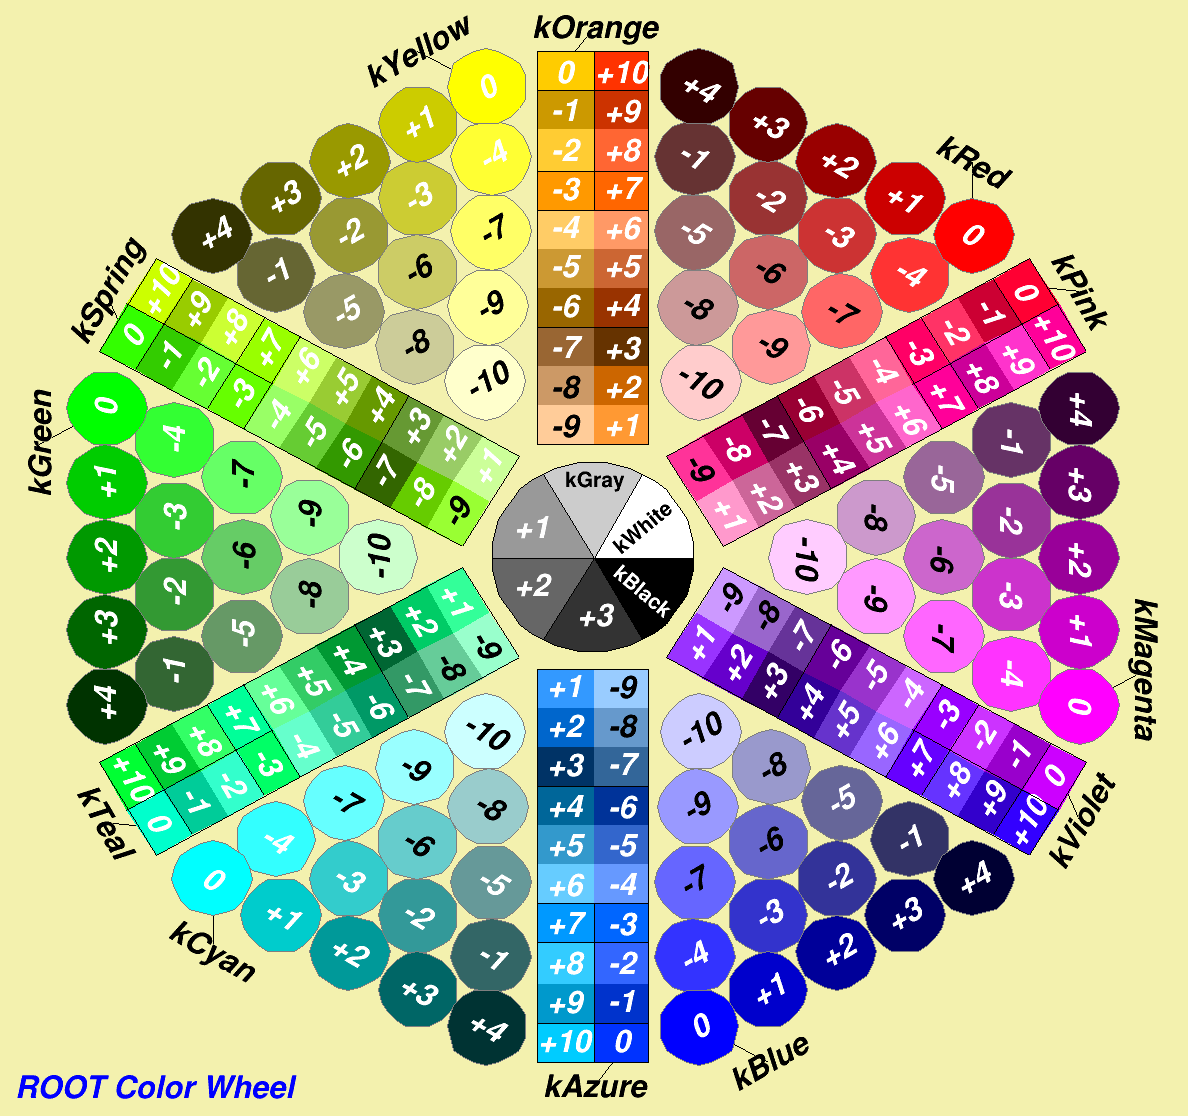
\includegraphics[scale=0.2]{imgs_root/maxres.png}
\end{figure}

\subsection{Drawing TGraph}
\begin{description}
\item[\ttt{graph->Draw(<options>)}]
\item[\ttt{"A"}] draws axis
\item[\ttt{"P"}] draws points markers (the current one set)
\item[\ttt{"E"}] draws error bars
\item[\ttt{"AI"}] draws invisible axis (no labels)
\item[\ttt{*}] draws star at each point (alternative to $P$)
\item[\ttt{C}] draws a smooth curve connecting points
\item[\ttt{X+}] X axis drawn on the top side
\item[\ttt{Y+}] Y axis drawn on the right side
\item[\ttt{RX}] reverse the X axis
\item[\ttt{RY}] reverse the Y axis
\end{description}
\subsection{Drawing TGraphErrors}
Along with previous options, some specific ones:
\begin{description}
\item[\ttt{Z}] do \textbf{not} draw horizontal and vertical lines at the end of error bars
\item[\ttt{>}] draw arrow at the end
\item[\ttt{|>}] filled arrow
\item[\ttt{X}] do \textbf{not} draw error bars
\item[\ttt{||}] draw only lines at the end of bars, \textbf{not} bars themselves
\item[\ttt{0}] force error bars drawing also for points outside visible range along Y (by default they're not drawn)
\item[\ttt{2}] draw error rectangles
\item[\ttt{3}] filled area through the end points
\item[\ttt{4}] smoothed filled area
\item[\ttt{5}] like \ttt{2}, but countour lines are drawn.

\end{description}
\subsection{Additional styling}
\begin{description}
\item[\ttt{gStyle->SetErrorX(<dx>)}] if set to $0$ removes error along x
\item[\ttt{gStyle->SetEndErrorSize(<n\_px>)}] size of line at the end of error bars. Default = $1$.
\end{description}

\section{Fit}
The following syntax is valid both for histos and graphs.
\begin{description}
\item[\ttt{<pt>->Fit( "<name>", "<option>", "<graphic\_opt>", <xmin>, <xmax>);}] \,\\where \ttt{name} is one of the defaults: 
\begin{description}

\item[\ttt{gaus}] \ttt{gausn} (normalized)

\item[\ttt{landau}] \ttt{landaun} \ttt{expo} \ttt{pol1} \ttt{pol2} ... \ttt{pol9} (polynomial of degree $n$)

\item[\ttt{chebyshev1}] \ttt{chebyshev2} ... \ttt{chebyshev9}

\end{description}

To print list of avaiable functions: \begin{verbatim}
TF1::InitStandardFunctions(); // not needed if `gROOT->GetFunction()` is called before
gROOT->GetListOfFunctions()->ls();
\end{verbatim}

\ttt{name} can also be a formula accepted by the linear fitter with the operator \ttt{++}\\
(e.g. \ttt{x++sin(x)}, for fitting \ttt{[0]*x+[1]*sin(x)})
\item[\ttt{<pt>->Fit( TF1* f1,"<option>","<graphi\_opt>",<xmin>,<xmax>)}] with previously defined function (see after)
\end{description}
\ttt{graphic\_opt} is analogous to the one for \ttt{Draw}, whereas \ttt{option} can contain one (or more) of the following:
\begin{description}
\item[FOR HISTOS ONLY]
\item[\ttt{L}] use logarithmic likehood method (instead of default Chi square)

\item[\ttt{WIDTH}] scales histogram bin content by bin width (useful for variable bins)
\item[\ttt{MULTITHREAD}] forces employment of multithreading whenever possible
\item[FOR GRAPHS ONLY]
\item[\ttt{W}] ignore point errors when fitting TGraphErrors
\item[FOR BOTH HISTOS AND GRAPHS]
\item[\ttt{R}] use fitting range specified in the function range (default is histo's)
\item[\ttt{C}] in case of linear fit, disables calculation of Chi square (saves CPU time)
\item[\ttt{Q}] quiet mode: print minimum data
\item[\ttt{V}] verbose mode: print everything
\item[\ttt{S}] stores full fit result and returns a \ttt{TFitResultPtr} for access
\end{description}

\begin{description}
\item[\ttt{TF1* fitFunc = <pt>->GetFunction("f1")}] recover fit function from histo (analogous for graph)
\item[\ttt{fitFunc->GetChisquare()}]
\item[\ttt{fitFunc->GetNDF();}] degrees of freedom
\item[\ttt{fitFunc->GetParameter(<i>);}] \ttt{i}-th parameter value
\item[\ttt{fitFunc->GetParError(<i>);}] error on \ttt{i}-th parameter
\item[ONLY IF "S" OPTION USED:]
\end{description}
\begin{verbatim}
TFitResultPtr r = h->Fit(“fitFunc", “S”); 
TMatrixD cor = r->GetCorrelationMatrix();
TMatrixD cov = r->GetCovarianceMatrix();
cor.Print();
cov.Print();
\end{verbatim}

\subsection{Statistics \& fit parameters}
\ttt{gStyle->SetOptStat(<ksiourmen>)} choose statistics parameters to be displayed \\
(each mode with a value - default \textbf{0} if omitted):
\begin{itemize}
\item[\ttt{k}] \textbf{1} = print kurtosis, \textbf{2} = print kurtosis + k. error
\item[\ttt{s}] \textbf{1} = print skewness, \textbf{2} = print skewness + s. error
\item[\ttt{i}] \textbf{1} =print integral of bins, \textbf{2} = print integral of bins with option 
\item[\ttt{o}] \textbf{1} = print number of overflows
\item[\ttt{u}] \textbf{1} = print number of underflows
\item[\ttt{r}] \textbf{1} = print SD \textbf{2} = print SD + SD error \footnote{Actually \ttt{r} stands for Root Mean Square, defined according to 
\[x_{RMS} = \sqrt{\frac{1}{n} \sum x_i^2}\]
} 
\item[\ttt{m}] \textbf{1} = print mean \textbf{2} = print mean + mean error
\item[\ttt{e}] \textbf{1} = print number of entries
\item[\ttt{n}] \textbf{1} = print histogram name 
\end{itemize}
\textbf{STARTS FROM THE END:} 
\begin{verbatim}
gStyle->SetOptStat(11); // only name + entries
gStyle->SetOptStat(1101); // name, mean, RMS
\end{verbatim}
\ttt{gStyle->SetOptFit(<pcev>)} analogous for fit parameters:
\begin{itemize}
\item[\ttt{p}] \textbf{1} = print Probability
\item[\ttt{c}] \textbf{1} = print Chisquare / Number of d.o.f.
\item[\ttt{e}] \textbf{1} = print errors
\item[\ttt{v}] \textbf{1} = print name/values of parameters (only non-fixed) \textbf{2} = print name/value of \textit{all} parameters
\end{itemize}
\ttt{gStyle->SetOptFit(1)} is \textbf{equivalent} to \ttt{gStyle->SetOptFit(111)} (!)

\section{Functions}
In 1 variable (x): class \textbf{TF1}. User-defined function (and function objects, lambda) or built-in function objects $\rightarrow$ \textbf{TFormula}
\\For more dimensions (variables) \textbf{TF2, TF3}.
\begin{description}
\item[\ttt{TF1 *f1 = new TF1("f1", "sin(x)/x",<xmin>,<xmax>);}]
\item[\ttt{TF1 *f2 = new TF1("f2", "f1 * 2",0,10);}] previously defined functions can be used in definition of new ones
\item[\ttt{TF1 *f3 = new TF1("f3","[0]*x*sin([1]*x)",-3,3);}] possible to use parameters
\item[\ttt{f3->SetParameter(<index>, <value>);}] to \textbf{initialize} one of them
\item[\ttt{f3->SetParameters(<value1>, <value2>, ..., <valuek>);}] following order!
\item[See TFormula] for more info
\end{description}
For user-defined:
\begin{verbatim}
Double_t MyFunction(Double_t *x, Double_t *par){ 
    Float_t xx = x[0];
    Double_t val = TMath::Abs(par[0]*sin(par[1]*xx)/xx); 
    return val;
}
\end{verbatim}
\textbf{Note:} important to follow this signature!
\begin{description}
\item[\ttt{TF1 *f4 = new TF1("f4",MyFunction,0,10,2);}] {}\,\\
last constructor parameter is \textbf{number of parameters in MyFunction}
\item[\ttt{TF1 *f5 = new TF1("f5", [](double *x, double *p)\{ <function body> \}, <xmin>, <xmax>, <npar>);}] use of lambdas is also possible
\item[\ttt{TF1 *f6 = new TF1("f6", "[](double *x, double *p)\{ <function body> \}", <xmin>, <xmax>, <npar>);}] also as string expression (JIT will do the rest)
\end{description}
\paragraph{Cosmetics}
\begin{description}
\item[\ttt{f1->SetLineColor(kRed);}]
\item[\ttt{f1->SetLineStyle(2);}] 2 = dashed, 3 = dotted, 4 = dasheddotted
\end{description}
\paragraph{Member functions:}
\begin{description}
\item[\ttt{f1->Eval(<x\_value>);}] evaluate on a point
\item[\ttt{f1->Integral(<a>, <b>);}] compute $\displaystyle \int_a^b f1$
\item[\ttt{f1->SetMaximum(<value>);}] set maximum for Y axis
\item[\ttt{f1->SetMinimum(<value>);}] minimum for Y axis
\item[\ttt{f1->SetRange( <x\_min> , <x\_max> );}] set interval for indipendent variable to \ttt{\big[x\_min,x\_max\big]}
\end{description}

\newpage
\section{TMath and TFormula}
\subsection*{TMath}
\begin{description}
\item[\ttt{TMath::Abs(<x>)}]
\item[\ttt{TMath::AreEqualAbs(<x>,<y>,<eps>)}]returns  true if \ttt{TMath::Abs(x-y) < eps}
\item[\ttt{TMath::ASin(<x>)}]; \ttt{TMath::ASinH(<x>); TMath::ATan(<x>); TMath::ACos(<x>); TMath::ACosH(<x>)}
\item[\ttt{TMath::Cos(<x>)}]; \ttt{TMath::CosH(<x>)}
\item[\ttt{TMath::Sin(<x>)}]; \ttt{TMath::SinH(<x>)}
\item[\ttt{TMath::Tan(<x>)}]; \ttt{TMath::TanH(<x>)}
\item[\ttt{TMath::Ln10()}] returns $\ln 10$
\item[\ttt{TMath::LogE()}] returns $\log_{10} e$
\item[\ttt{TMath::Ldexp(<x>, <exp>)}] where \ttt{exp} is integer. Returns $x \cdot 2^{exp}$
\item[\ttt{TMath::Log(<x>)}] natural logarithm
\item[\ttt{TMath::Log10(<x>)}] returns $\log_{10} x$
\item[\ttt{TMath::Log2(<x>)}] returns $\log_2 x$
\item[\ttt{TMath::Max(<x>,<y>)}] returns maximum value between \ttt{x} and \ttt{y}
(for integers, doubles... everything)
\item[\ttt{TMath::Min(<x>,<y>)}] same but for minimum
\item[\ttt{TMath::Nint(<x>)}] rounds \ttt{x} to mearest integer
\item[\ttt{TMath::Power(<x>,<y>)}] returns $\displaystyle x^y$
\item[\ttt{TMath::Prob(<chi2>,<ndof>)}] returns probability for $\chi^2$ = \ttt{chi2} with \ttt{ndof} degrees of freedom
\item[\ttt{TMath::Sq(<x>)}] returns $x^2$
\item[\ttt{TMath::Sqrt(<x>)}] returns $\sqrt{x}$
\item[CONSTANTS]
\item[\ttt{TMath::E()}] returns $e$
\item[\ttt{TMath::G()}] returns $G$
\item[\ttt{TMath::Gn()}] returns $g$
\item[\ttt{TMath::H()}] returns $h$ \ttt{TMath::Hbar()} returns $\hbar$
\item[\ttt{TMath::K()}] returns $k_B$
\item[\ttt{TMath::Na()}] returns $N_A$
\item[\ttt{TMath::Pi()}] returns $\pi$
\item[\ttt{TMath::R()}] returns $R$
\item[\ttt{TMath::Sigma()}] returns $\sigma$ (Stefan-Boltzmann)
\item[\ttt{TMath::Sqrt2()}] returns $\sqrt[•]{2}$
\end{description}
\subsection*{TFormula}
\begin{description}
\item[\ttt{gaus(<const>,<mean>,<sigma>)}] not normalized
\item[\ttt{landau(<mpv>,<sigma>)}]
\item[\ttt{expo(<const>,<slope>)}] $\displaystyle e^{A + Bx}$
\item[\ttt{pol<N>(<p1>, ... ,<pN>)}] polynomial $\displaystyle \sum_{i=1}^N pi \cdot x^i$ 
\item[\ttt{sqrt(<x>)}]
\item[\ttt{sq(<x>)}] $x^2$
\item[\ttt{pow(<x>,<y>)}] $x^y$
\item[\ttt{<x>*<y>}]
\item[\ttt{<x>\textasciicircum <n>}] or \ttt{<x>**<n>}
\item[\ttt{<x>/<y>}]
\item[\ttt{sin(<x>)}] \ttt{cos(<x>)} \ttt{tan(<x>)}
\item[\ttt{asin(<x>)}] \ttt{acos(<x>)} \ttt{atan(<x>)}
\item[\ttt{sinh(<x>)}] \ttt{cosh(<x>)} \ttt{tanh(<x>)}
\item[\ttt{asinh(<x>)}] \ttt{acosh(<x>)} \ttt{atanh(<x>)}
\item[\ttt{exp(<x>)}]
\item[\ttt{log(<x>)}]
\item[\ttt{log10(<x>)}]
\item[\ttt{e}] \quad \big| \quad \ttt{pi}
\item[\ttt{ln10}] \quad \big| \quad \ttt{sqrt2}
\end{description}
In function initialization, values can be replaced either with the variable \ttt{x} or parameters \ttt{[i]}.\\
Some special ones, where \textbf{\ttt{n} is the starting index for numbering.}
\begin{description}
\item[\ttt{gaus(<n>)}] not default normalized gaussian with three parameters
\item[\ttt{gausn(<n>)}] normalized gaussian with three parameters
\item[\ttt{expo(<n>)}] exponential with three parameters
\item[\ttt{pol<N>(<n>)}] polynomial with \ttt{N} parameters
\end{description}

\newpage
\section{Legend}
\ttt{TLegend *leg = new TLegend(<x1>,<y1>,<x2>,<y2>,"<title>");}
\\$(x1,y2)$ = bottom left corner, $(x2,y2)$ = upper right corner \textbf{in normalized coordinates} \\so $1$ = \textbf{pad} height / width
\[x = \frac{absolute \enspace horizontal \enspace position}{screen \enspace width} \qquad y = \frac{absolute \enspace vertical \enspace position}{screen \enspace height}\]
$x$ goes from left to right, $y$ from bottom to top\\
Careful when using more pads (see\textbf{ Canvas syntax})
\begin{verbatim}
leg->AddEntry(graph,"Punti sperimentali"); 
leg->AddEntry(f,"Fit Lineare"); 
leg->AddEntry(<object>,"<description>");
leg->AddEntry(<object>,"<description>", "<option>"); // alternative syntax
\end{verbatim}
Possible options (even more than one of these): 
\begin{description}
\item[\ttt{l}] line
\item[\ttt{e}] error bar
\item[\ttt{p}] point
\end{description}

\begin{verbatim}
leg->Draw("Same"); 
\end{verbatim}
\ttt{leg->SetTextAlign(<nm>);} with \texttt{nn} = 11, ..., 13 \hfill $\begin{array}{c|c|c} 11 & 21 & 31 \\\hline
12 & 22 & 32 \\\hline
13 & 23 & 33
\end{array}$

\paragraph{Cosmetics (\ttt{gStyle} member functions)}
\begin{verbatim}
gStyle->SetLegendBorderSize(<n>);
gStyle->SetLegendFillColor(<color>);
gStyle->SetLegendFont(<n>); // see below
gStyle->SetLegendTextSize(<size>); // see below
\end{verbatim}
\begin{center}
\textbf{font code (\ttt{<n>}) = 10 $\times$ font number + precision}
\end{center}
Example of fonts with precision $= 2$:
\begin{figure}[H]
\centering
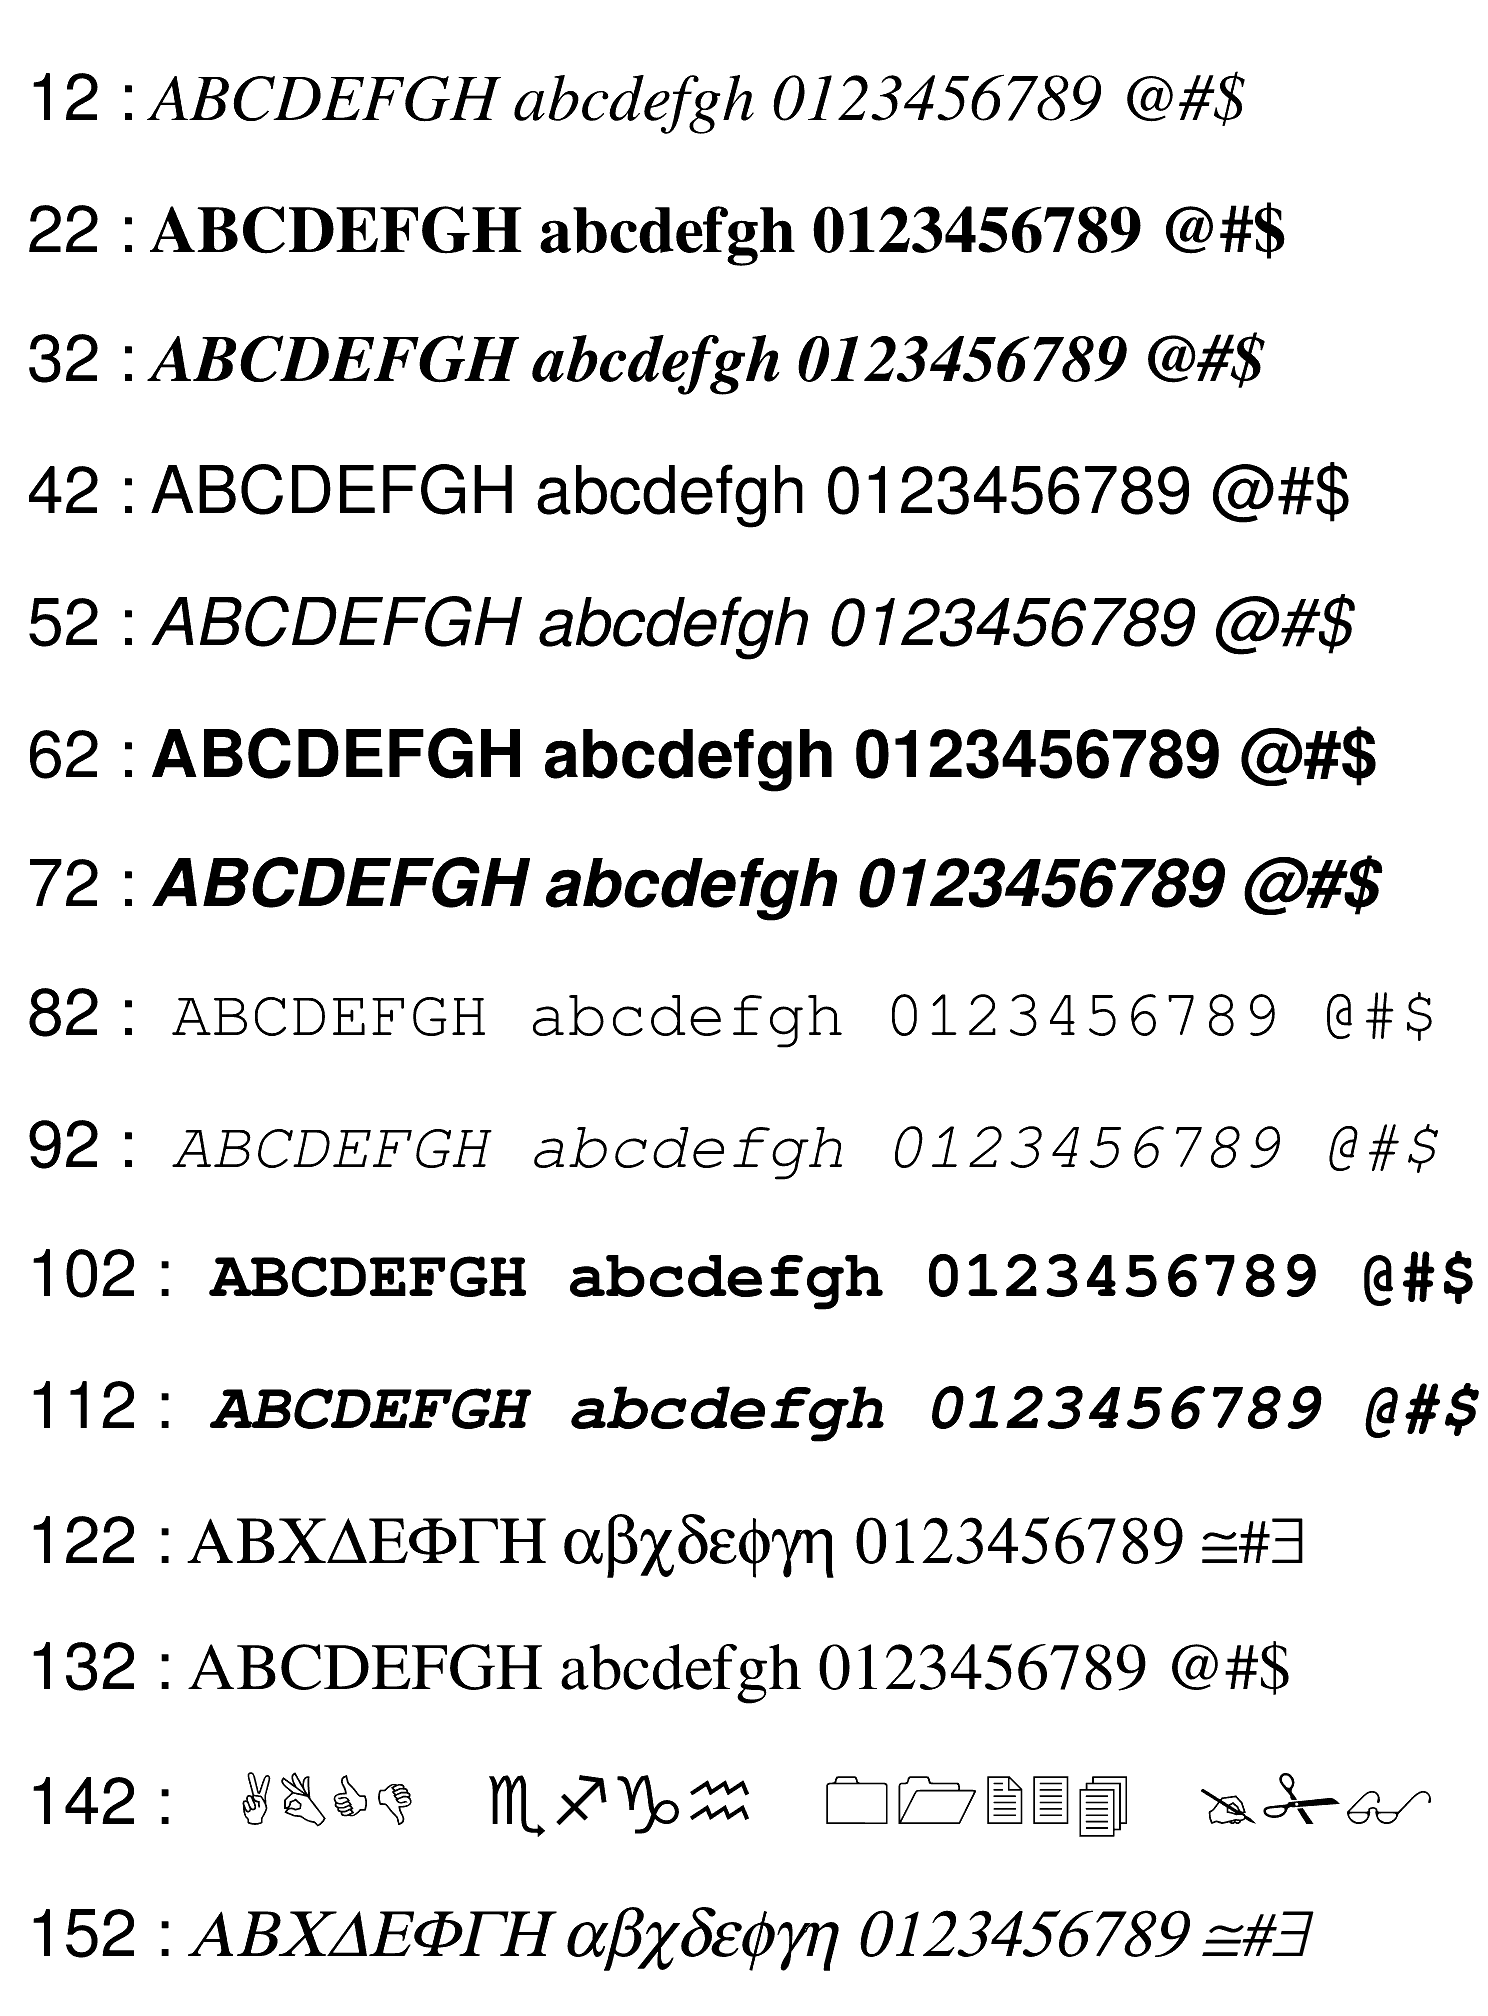
\includegraphics[scale=0.13]{imgs_root/fonts.png}
\end{figure}

\section{Canvas syntax}
\begin{description}
\item[\ttt{TCanvas* myCanvas = new TCanvas()}]
\item[\ttt{TCanvas* myCanvas = new TCanvas()}]
\item[\ttt{myCanvas->Print("<file-name>.<extension>", "<option>");}] prints canvas to file. Possible formats: 
\begin{description}
\item[\ttt{.ps}] (Postscript, default one) with options \ttt{Portrait} or \ttt{Landscape}, \item[\ttt{.eps}] (encapsulate Postscript), \ttt{.pdf} with option \ttt{Title: <title>}, \item[\ttt{.svg, .tex, .gif, .gif+<N>}] (animated gif, where \ttt{N} is the delay in units of 10ms)
\item[\ttt{.xpm, .png, .jpg, .tiff, .cxx, .xml, .json, .root}]
\end{description}

\item[\ttt{myCanvas->SetCanvasSize(<x\_px>,<y\_px>);}]
\item[\ttt{myCanvas->SetWindowSize(<x\_px>,<y\_px>);}]{}\,\\
If canvas size exceeds window size, scrollbars are displayed
\item[\ttt{myCanvas->GetWh();}] get value of window height
\item[\ttt{myCanvas->GetWw();}] get value of window width
\item[\ttt{myCanvas->ToggleToolBar();}] hides if shown or vice versa
\end{description}
\subsection*{Pads}
\begin{description}
\item[\ttt{myCanvas->Divide(<nx>, <ny>)}] divides equally into nx$\times$ny pads 
\item[\ttt{myCanvas->Divide(<nx>, <ny>, <x\_margin>, <y\_margin>, <color>)}] Same; margins are given as \textbf{percent of canvas}. \ttt{color} is the color of new pads; 
\end{description}
Pads can be divided in sub-pads.
\begin{description}
\item[\ttt{myCanvas->cd(<pad\_num>)}] sets current pad. Starts from \ttt{1}, \ttt{0} is parent pad (frame). Current pad can be retrieved through \ttt{gPad}. It goes by rows, so the numbering looks like:
\end{description}
\[\begin{bmatrix}
1 & \rightarrow &  n \\
n+1 & \rightarrow & 2n \\
\vdots & \vdots & \vdots\\
(m-1)n + 1 & \rightarrow & mn
\end{bmatrix}\]
\newpage
\section{Pseudo-Random number generation: TRandom}
Classes with algorithms employed:
\begin{itemize}
\item \texttt{TRandom \, \dotfill \, Linear Congruential Generator}
\begin{center}
\boxed{\textit{ $\nwarrow$ It's a \textbf{very bad} generator, not to be used!}}
\end{center}
\item \texttt{TRandom1 \, \dotfill \, RANLUX}
\item \texttt{TRandom2 \, \dotfill \, Tausworthe}
\item \texttt{TRandom3 \, \dotfill \, Mersenne Twister}
\end{itemize}
\subsection{Methods for generic distributions}
Called on global pointer \ttt{gRandom} or on \ttt{TRandom*} pointer after declaration
\begin{description}
\item[\ttt{Uniform(<double\_1>, <double\_2>)}] uniform distribution on \ttt{\big]double\_1, double\_2\big]} based on \ttt{Rndm()}
\item[\ttt{Rndm()}] uniform in \ttt{\big]0, 1\big]}
\item[\ttt{Uniform(<double>)}] uniform distribution on \ttt{\big]0, double\big]}
\item[\ttt{Integer(<int\_max>)}] uniform \textbf{integer} distribution on \ttt{\big[0, int\_max - 1\big]}
\item[\ttt{Gaus(<mean>, <sigma>)}] (careful, just one '\ttt{s}')
\item[\ttt{Poisson(<mean>)}] \textbf{integer} poissonian distribution
\item[\ttt{PoissonD(<mean>)}] \textbf{double} poissonian distribution
\item[\ttt{Binomial(<n\_tot>, <prob\_of\_succ>)}]
\item[\ttt{Exp(<tau>)}]
\item[\ttt{Landau(<mpv>, <sigma>)}] Landau distribution: \ttt{mpv} is the \textit{most probable value} (moda) and sigma is \textit{not} the SD (which is undefined)
\end{description}

\subsection{Random generation from a generic function}
\begin{verbatim}
TF1 *f1 = new TF1("f1", "<expression>", <xmin>, <xmax>);
double rd = f1->GetRandom();
\end{verbatim}
\ttt{r} is now a random variable distributed according to the PDF defined by \ttt{f1}. It is not necessary to manually ensure that \ttt{f1} is normalized: \textbf{normalization is carried out automatically}, the only requirement on the function is \textbf{continuity}.
\begin{description}
\item[\ttt{histo->FillRandom("<function>", <n>)}] fills the histogram with \ttt{n} extractions from a random variable distributed according to \ttt{f1} (name). Same considerations as before apply.
\end{description}
\subsection{Filling an histo with randomly generated values}
\begin{verbatim}
for(Int_t j=0;j<ngen;j++){ // generation loop
   Double_t x = gRandom->Uniform(xmin,xmax); // extraction
   h->Fill(x); // filling
}
\end{verbatim}

\section{Benchmark}

\begin{description}

\item[\ttt{TBenchmark *b = new TBenchmark();}] initialize

\item[\ttt{b->Start("<name>");}] start benchmark with specified name 
\\(more with different names from same \texttt{b})

\item[\ttt{b->Stop("<name>");}] stop benchmark with specified name

\item[\ttt{b->Print("<name>");}] print parameters

\item[\ttt{b->Show("<name>");}] = \texttt{stop} + \texttt{print}

\end{description}

\section{Trees}
Data structures for storage of homologous units made of \textit{heterogeneous} objects. Useful for data persistance, optimization of memory usage (thanks to compression) and I/O speed - expecially in WORM - and flexibility in analysis.
\\Can handle \textbf{any} data type. Direct access to any point; only object (even partially) placed on memory.
\\Organised in \texttt{TBranch}es, themselfs structured in \texttt{TLeaf}s

\subsection{Filling}
\begin{verbatim}
TTree *T = new TTree("T","test"); // create the tree 
Float_t x,y,z;
T->Branch("x",&x,"x/F"); // create branches 
T->Branch("y",&y,“y/F"); // <name>/<type>
T->Branch("z",&z,“z/F"); 
for(Int_t i=0;i<100;i++){
  ... // read or generate x y z, very costly operations
  T->Fill(); // fill the tree, for each entry
}
\end{verbatim}

\subsection{Reading and representing}
\begin{verbatim}
T->Print(); // list of contained variables

T->Draw(“x”); // show variable. Histo layout chosen by ROOT

TH1F *h1=new TH1F("h1","hist from tree",50,-4, 4); 
T->Draw("x>>h1"); // to fill user defined histo

T->Draw("x”,”x>0”);        // selection on 1v
T->Draw("x”,”y>0 && x<10”) // selection on 2vv

Tout->Draw(“sqrt(x*x+y*y)”); // operation on variables

T->Draw(“y:x”);   // 2d correlation plot
T->Draw(“z:y:x”); // 3d
\end{verbatim}








\end{document}
